\documentclass{article}
\usepackage{titling}
\usepackage{parskip}
\usepackage{setspace}
\usepackage[utf8]{inputenc}
\usepackage{amsmath, amsthm, amssymb, amsfonts, mathtools, xfrac, dsfont}
\usepackage[labelfont=bf]{caption}
\usepackage[labelfont=bf]{subcaption}
\usepackage{float}
\usepackage[margin=0.8in]{geometry}
\usepackage{algorithm}
\usepackage{algorithmic}
\usepackage{xcolor}
\usepackage[export]{adjustbox}
\usepackage{hyperref}
\usepackage{tabularx}
\usepackage{makecell}
\usepackage{bm}
\usepackage{indentfirst}

\newcommand{\norm}[1]{\left\lVert#1\right\rVert}
\newcommand{\abs}[1]{\left|#1\right|}
\newcommand{\mat}[1]{\begin{bmatrix}#1\end{bmatrix}}
\renewcommand{\vec}[1]{\mathbf{#1}}
\renewcommand{\arraystretch}{1.3}
\newcommand{\R}{\mathbb{R}}
\newcommand{\Z}{\mathbb{Z}}
\newcommand{\E}{\mathbb{E}}
\newcommand{\N}{\mathcal{N}}
\DeclareMathOperator{\Cov}{Cov}
\DeclareMathOperator{\diag}{diag}
\DeclarePairedDelimiter\floor{\lfloor}{\rfloor}
\DeclarePairedDelimiter\ceil{\lceil}{\rceil}
\DeclareMathOperator*{\argmax}{arg\,max}
\DeclareMathOperator*{\argmin}{arg\,min}

\captionsetup{justification=centering}
\numberwithin{equation}{section}
\setlength\parindent{0.25in}
\setstretch{1.1}

\title{\textbf{Scalable Global Parameter Estimation for Nonstationary Gaussian Processes}}
\date{}
\author{
Paul G. Beckman\thanks{Mathematics and Computer Science Division, Argonne National Laboratory} \and
Christopher J. Geoga\footnotemark[1] \thanks{Department of Statistics, Rutgers University} \and
Mihai Anitescu\footnotemark[1] \thanks{Department of Statistics, University of Chicago}
}

\begin{document}

\maketitle

\vspace{-2\baselineskip}

\begin{abstract}
Put the abstract here.
\end{abstract}

\section{Introduction}

\begin{equation}
  -\ell(\bm{\theta}) := \frac{1}{2}\log\abs{\bm{\Sigma}(\bm{\theta})} + \frac{1}{2}(\mathbf{y}-\bm{\mu})^\top\bm{\Sigma}(\bm{\theta})^{-1}(\mathbf{y}-\bm{\mu}) + \frac{n}{2}\log(2\pi)
  \label{nll}
\end{equation}

Minimizing \ref{nll} numerically can be computationally expensive, as conventional determinant and linear solve operations scale cubically in time and quadratically in storage. As $n$ grows, the evaluation of \ref{nll} thus becomes prohibitively expensive. In response to these scaling challenges, a number of methods have been introduced to more efficiently compute or approximate \ref{nll}.

Fast Gaussian process MLE methods (Vecchia, Guinness, Chen-Stein, Anitescu-Stein, Lindgren, Minden, Geoga, Ambikasaran)

We choose to use HODLR

With the exception of \cite{guinness2019gaussian}, all of these scalable methods are applied to stationary models. However, stationarity is often an unrealistic assumption for large datasets spanning spatial regions in which small scale dynamics cause variation in the local behavior of the data. To address this issue, past work has used locally stationary models in which the parameters of the random field are assumed to be constant in some neighborhood. Both disjoint neighborhoods \cite{lenzi2019improving} and overlapping or moving window neighborhoods \cite{kuusela2018locally, anderes2011local} have been used for maximum likelihood parameter estimation and prediction. Under such approaches, one must perform parameter estimation and prediction using only the observations lying in a single neighborhood instead of using the entire set of observations, as the stationary GP model is only assumed locally. Thus one must choose the neighborhood size a priori to balance the spatial scale of the nonstationary with the density of observations such that the neighborhoods are small enough to capture local variation but contain sufficient observations to make accurate predictions. The scalability of matrix operations using the HODLR-approximated covariance $\bm{\tilde{\Sigma}}$ allows us to use the full dataset for parameter estimation and prediction, sidestepping the question of neighborhood size.

Convolution framework

Apart from locally stationary models, significant effort has been devoted to the construction of positive definite nonstationary covariance functions with spatially varying parameters. Gibbs \cite{gibbs1997bayesian} derives a squared exponential covariance function with a spatially varying range. Paciorek \cite{paciorek2003nonstationary} generalizes this result to allow spatially varying anisotropy for arbitrary stationary covariance functions. Stein \cite{stein2005nonstationary} introduces the following Mat\'ern covariance function with spatially varying anisotropy $\Lambda : \Omega \to \mathbb{S}^d_{++}$, variance $\sigma^2 : \Omega \to \R_+$, and smoothness $\nu : \Omega \to \R_+$
\begin{equation}
  k(\mathbf{x}_i, \mathbf{x}_j; \bm{\theta}) := \sigma^2(\mathbf{x}_i) \sigma^2(\mathbf{x}_j) \abs{\frac{\Lambda(\mathbf{x}_i) + \Lambda(\mathbf{x}_j)}{2}}^{-\frac{1}{2}}
  \mathcal{M}_{\frac{\nu(\mathbf{x}_i) + \nu(\mathbf{x}_j)}{2}} \bigg( \sqrt{Q_{ij}} \bigg)
  \label{kernel}
\end{equation}
using the quadratic form
\begin{equation*}
  Q_{ij} := (\mathbf{x}_i - \mathbf{x}_j)^\top \Big(\frac{\Lambda(\mathbf{x}_i) + \Lambda(\mathbf{x}_j)}{2}\Big)^{-1} (\mathbf{x}_i - \mathbf{x}_j),
\end{equation*}
where $\mathcal{M}_\nu$ is the stationary isotropic Mat\'ern covariance function
$$ \mathcal{M}_\nu(r) := \frac{2^{1-\nu}}{\Gamma(\nu)} (\sqrt{2\nu} r)^\nu K_\nu(\sqrt{2\nu} r) $$
and $K_\nu$ is the modified Bessel function of the second kind of order $\nu$.

In order to compute the nonstationary covariance function \ref{kernel}, one must specify the functions $\Lambda, \sigma^2,$ and $\nu$. A number of nonparametric and semiparametric methods have been proposed in the literature to construct global approximations to these nonstationary parameter functions. Risser et al. impose parametric forms with respect to covariate data \cite{risser2015regression}. Paciorek et al. \cite{paciorek2004nonstationary} propose a hierarchical Bayesian model for a nonstationary anisotropy matrix in which the eigenvalues and Givens angles of the eigenvector matrix are given stationary GP priors.
Noting that observations from a GP can be expressed as a linear combination of $n$ radial basis functions (RBFs) with centers $c_i$ fixed at the observations and shapes $\varphi(\norm{\mathbf{x} - \mathbf{c}_i}) = k(\mathbf{x}, \mathbf{c}_i)$ defined by the covariance function, the authors employ a low-rank GP approximation with a set of $k \leq n$ \textit{knots} on a coarse grid over a two-dimensional spatial domain which serve as a reduced set of RBF centers \cite{kammann2003geoadditive, paciorek2006spatial}.

Additional work has been done with explicit RBF representations of nonstationary parameters. Gibbs \cite{gibbs1997bayesian} uses a linear combination of RBFs on a one-dimensional grid to estimate a nonstationary range parameter, using Gaussian priors on the basis function weights. Guinness \cite{guinness2019gaussian} uses a set of orthogonalized RBFs to approximate a nonstationary scale parameter. Finally, Higdon \cite{higdon1998process} and Paciorek \cite{paciorek2003nonstationary} employ a normalized RBF approximation in which the nonstationary parameters are computed as RESTRUCTURE FOR OTHER REFERENCES
\begin{equation}
  \bm{\theta}(\mathbf{x}) := \frac{\sum_{i=1}^m \varphi(\norm{\mathbf{x} - \mathbf{c}_i}) \ \bm{\theta}_i}{\sum_{i=1}^m \varphi(\norm{\mathbf{x} - \mathbf{c}_i})},
  \label{NRBF}
\end{equation}
where $\varphi$ is a radial function with radius parameter $\lambda$ and each $\bm{\theta}_i$ is a scalar- or matrix-valued variable representing a local parameter value at the RBF center $\mathbf{c}_i$. One can view \ref{NRBF} as a linear smoother of local parameter values, yielding a global parametric approximation to the nonstationary parameter. Minimizing \ref{nll} thus results in an $O(m)$-dimensional nonlinear optimization problem, which may include semidefinite or box constraints depending on the parameterizations of $\Lambda, \sigma^2,$ and $\nu$.

With the exception of the work by Guinness, which uses Fisher scoring to perform maximum likelihood estimation, all of the above methods use MCMC to sample the posterior distribution. Our main contribution is to introduce and test a number of scalable numerical optimization routines which are applicable to nonstationary parameter function approximations. In this way we provide flexible MLE alternatives to MCMC for a broad class of nonstationary models.

\section{HODLR matrices and scalable likelihood computations} \label{HODLR}
We now provide a brief overview of HODLR matrices and methods for computing the likelihood and its gradient and hessian in quasilinear time. A symmetric HODLR matrix is of the form
\begin{equation}
  \mat{A_1 & UV^\top \\ VU^\top & A_2}
  \label{HODLR}
\end{equation}
where $U, V \in \R^{n \times p}$ and $A_1$ and $A_2$ are either dense or of the form \ref{HODLR}.

% \begin{align*}
%   y &= L \bm{\omega} \\
%   \bm{\Sigma} &= LL^\top \\
%    \bm{\omega} &\sim \mathcal{N}(0, I)
% \end{align*}
% with the

\section{Computational considerations}
Although the HODLR approximation greatly improves the scalability of the evaluation of the likelihood and its derivatives, the nonlinear program \ref{} becomes high-dimensional and costly when a large number of anchors are used. We now discuss methods which improve the computational complexity of solving \ref{}.

\subsection{Compactly-supported basis functions}
scaling overview

O(m) to O(a) kernel evaluation

Although Gaussian RBFs truncated at some radius $\lambda$ would yield a similar sparse representation, we choose to employ compactly-supported basis functions because we can enforce an arbitrary level of smoothness at the origin and at $r=\lambda$. This allows us to maintain the $\floor{\nu}$-times mean-squared differentiability of the GP.

It is worth emphasizing that the use of a compactly-supported basis function to approximate the nonstationary parameter functions does not result in a compactly-supported kernel.

\begin{equation}
  \bm{\Sigma}_{jk} = K \mat{I_s \\ 0} + \mat{I_s & 0}\tilde{K}^\top
\end{equation}
where $K, \tilde{K} \in \R^{n \times s}$ are defined by
\begin{align*}
  K_{ij} &= k(\mathbf{x}_i, \mathbf{x}_j) \\
  \tilde{K}_{ij} &=
\end{align*}

\subsection{Scalable optimization}
Complexity of likelihood, gradient, and Hessian

Complexity of compact RBFs

Cholesky and SDP anisotropy formulations
\begin{align*}
  \min_{\Lambda_1, ..., \Lambda_k}  -\ell&(\Lambda_1, ..., \Lambda_k) \\
  \text{s.t.} \quad \Lambda_i & = \Lambda_i^\top \\
  \Lambda_i & \succeq 0 \quad \\
  \forall \ i & = 1,...,k \\
\end{align*}

Off-diagonal decay of Hessian

Unconstrained univariate nonstationary scale
\begin{itemize}
  \item COBYLA
  \item BFGS
  \item Full Hessian trust region
  \item Block diagonal Hessian trust region
  \item Full Fisher trust region
  \item Block diagonal Fisher trust region
\end{itemize}

\section{Numerical experiments} \label{experiments}
Parameter reconstruction with confidence intervals

Asymptotic results utilizing the orthogonality of Gaussian measures establish that even in the stationary case in which $\nu$ is fixed, the anisotropy $\Lambda = \alpha I$ is a scaling of the identity matrix, and the scale $\sigma^2 = \beta$ is a constant, the parameters $\alpha$ and $\beta$ cannot be consistently estimated simultaneously using an increasing number of observations in a fixed domain \cite{zhang2004inconsistent}.

\begin{figure}[t!]
  \begin{subfigure}[t]{0.5\textwidth}
    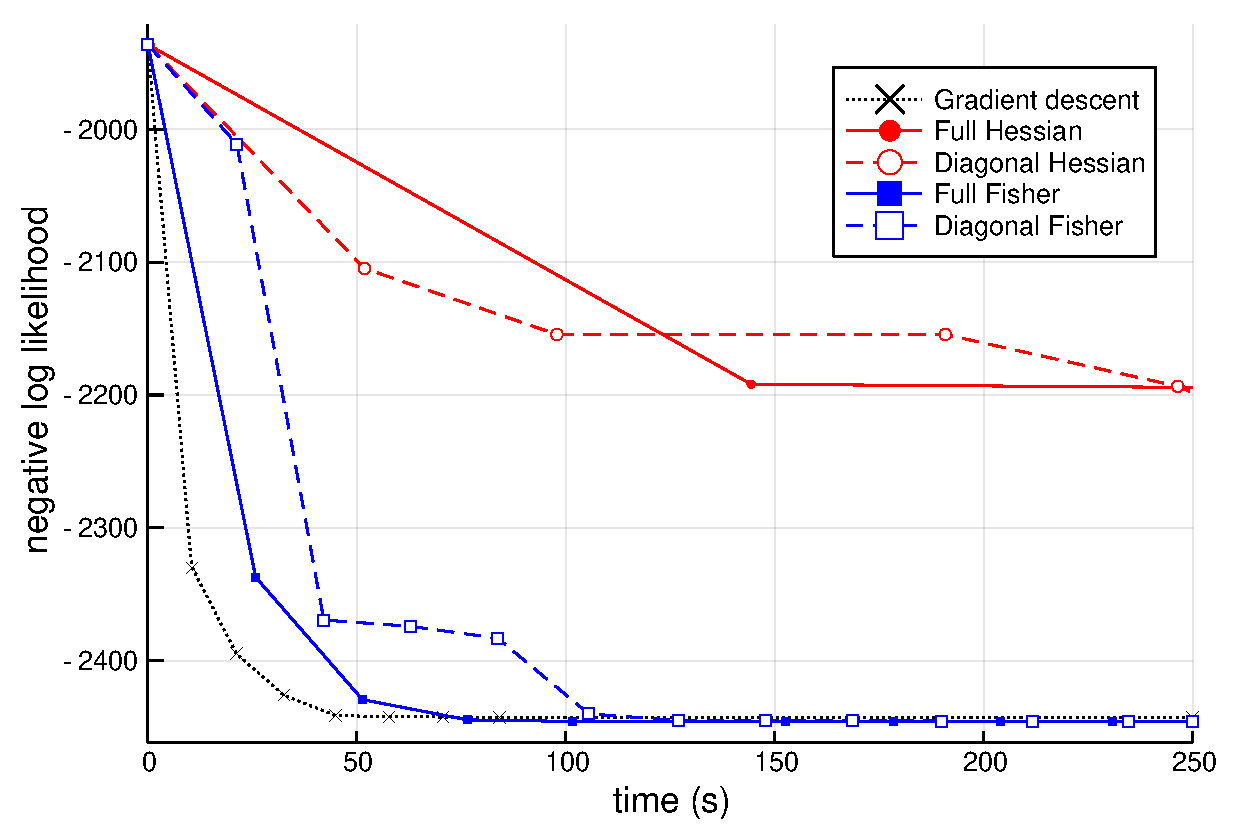
\includegraphics[width=\textwidth]{figures/timing/p1000-a20-plot.pdf}
    \caption{1000 observations with 20 anchors}
  \end{subfigure}%
  \begin{subfigure}[t]{0.5\textwidth}
    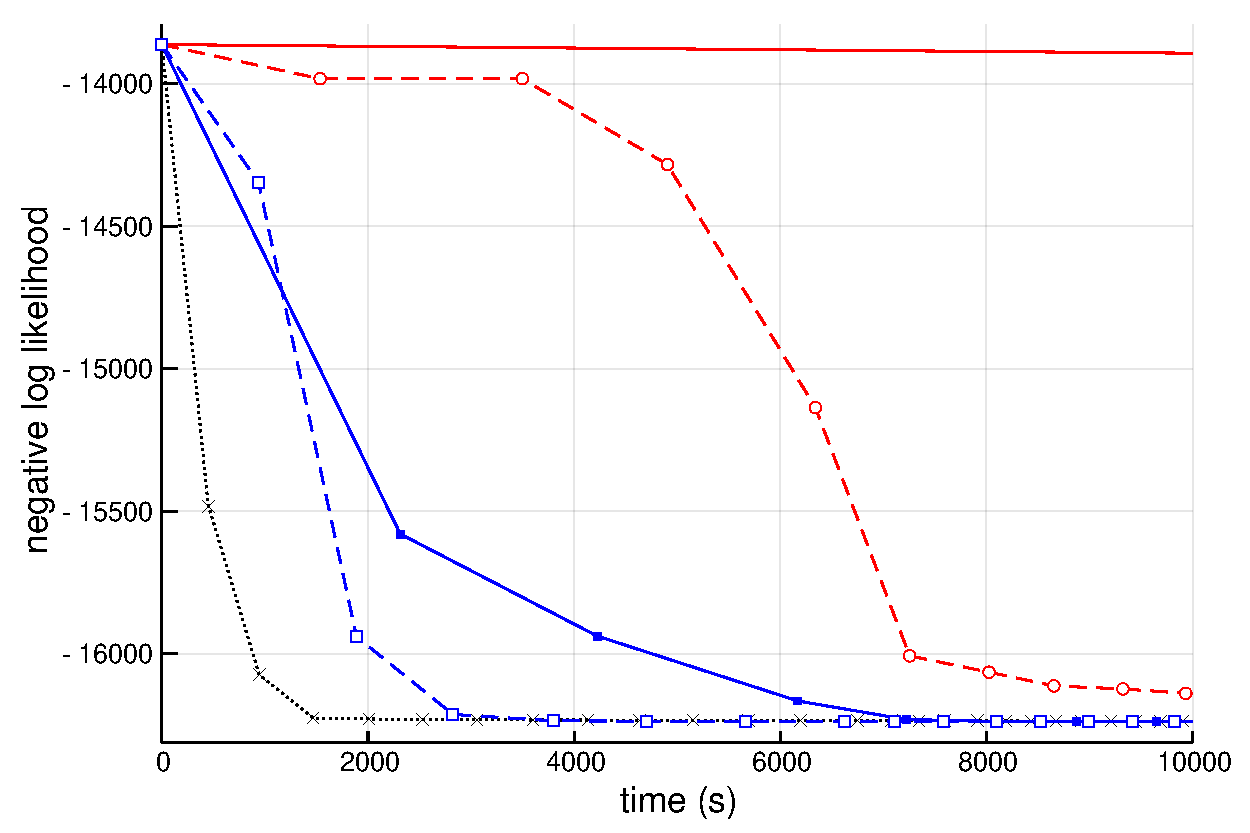
\includegraphics[width=\textwidth]{figures/timing/p5000-a50-plot.pdf}
    \caption{5000 observations with 50 anchors}
  \end{subfigure}
  \caption{Runtime comparison of gradient descent, Newton's method using the full Hessian and its diagonal, as well as Fisher scoring using the full Fisher-information matrix and its diagonal.}
\end{figure}

\begin{figure}[t!]
  \centering
  \begin{tabular}{cc}
    \begin{subfigure}[t]{0.3\textwidth}
      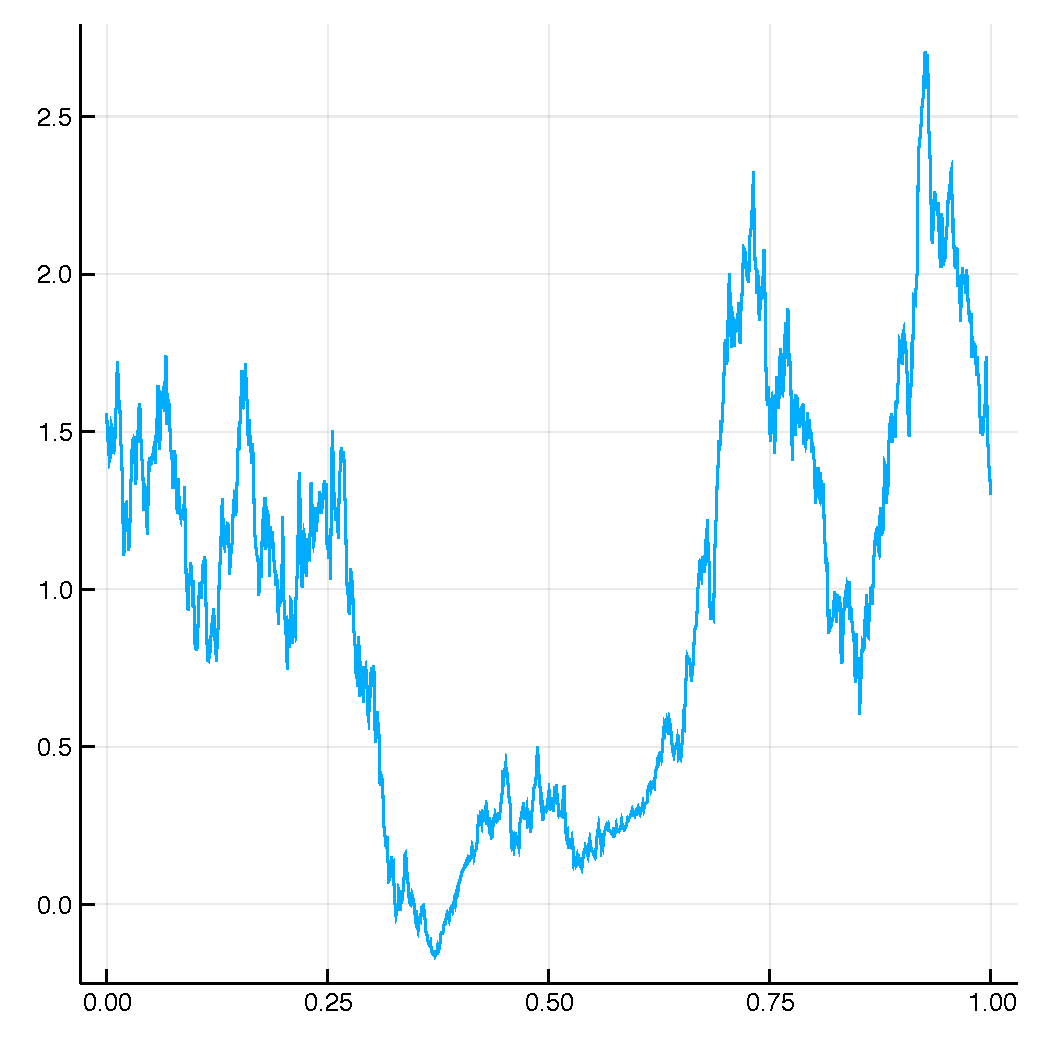
\includegraphics[width=\textwidth]{figures/scale/dat-nss-p1000.pdf}
      \caption{Simulated random field}
    \end{subfigure} &
    \begin{subfigure}[t]{0.3\textwidth}
      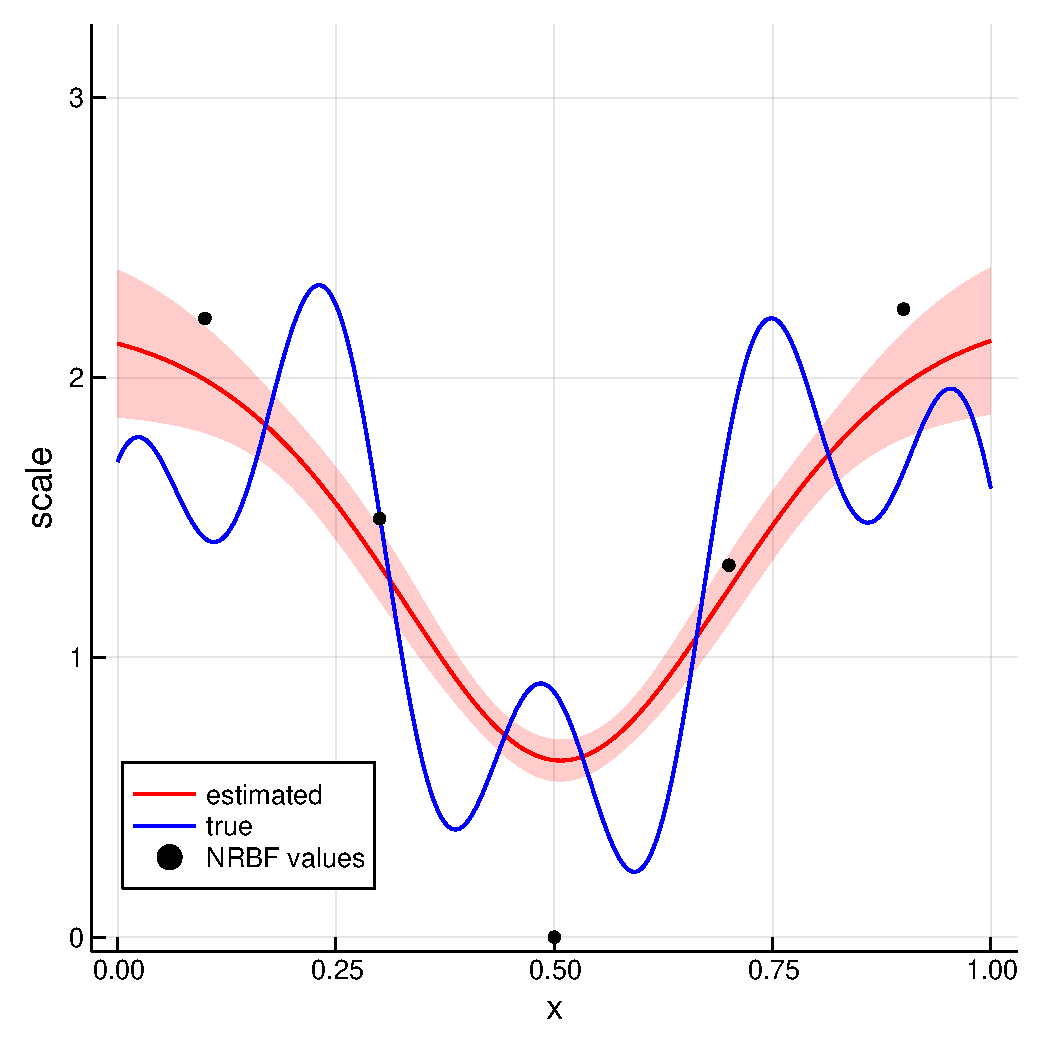
\includegraphics[width=\textwidth]{figures/scale/est-p1000-a5-se1.pdf}
      \caption{True and estimated scale function using 5 NRBFs}
    \end{subfigure}
    \\[4ex]
    &
    \begin{subfigure}[t]{0.3\textwidth}
      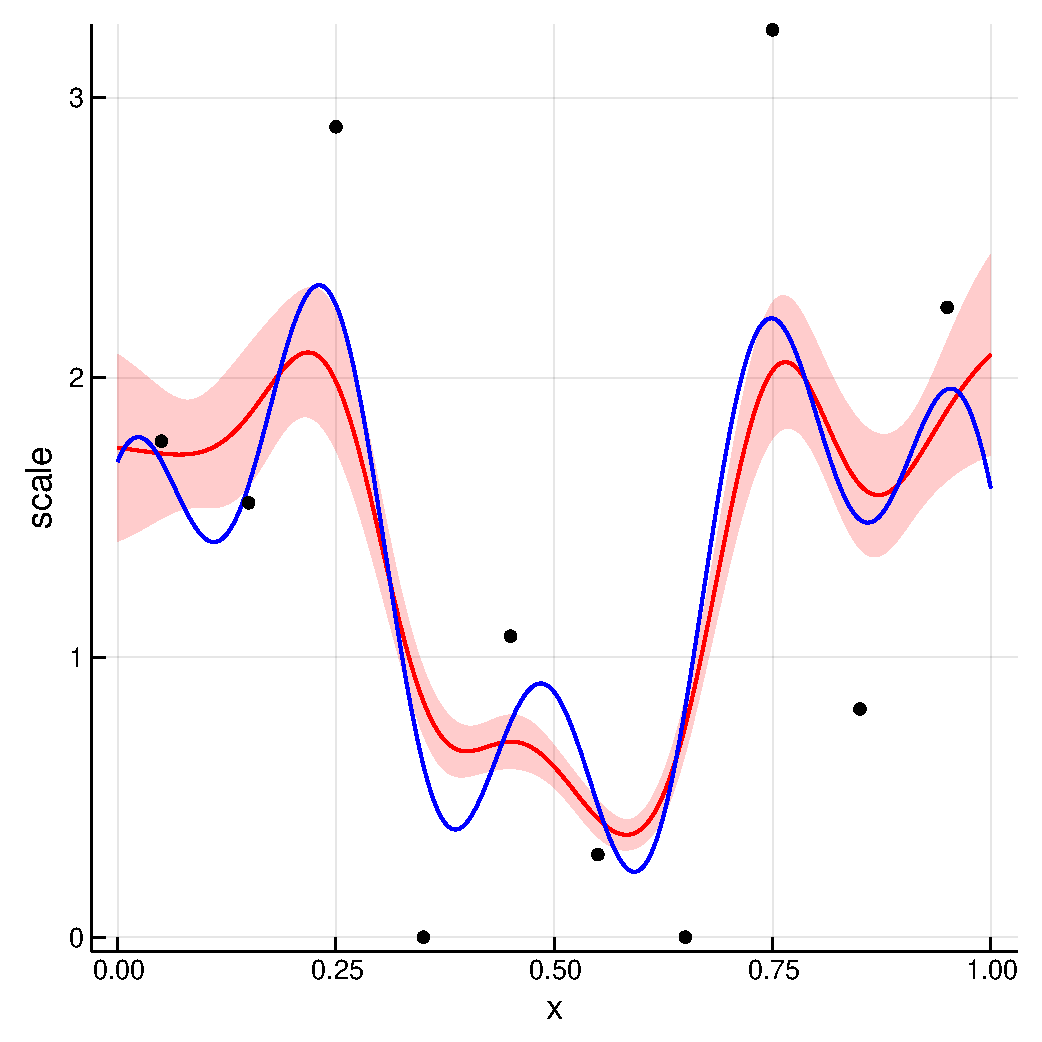
\includegraphics[width=\textwidth]{figures/scale/est-p1000-a10-se1.pdf}
      \caption{True and estimated scale function using 10 NRBFs}
    \end{subfigure}
    \\[4ex]
    &
    \begin{subfigure}[t]{0.3\textwidth}
      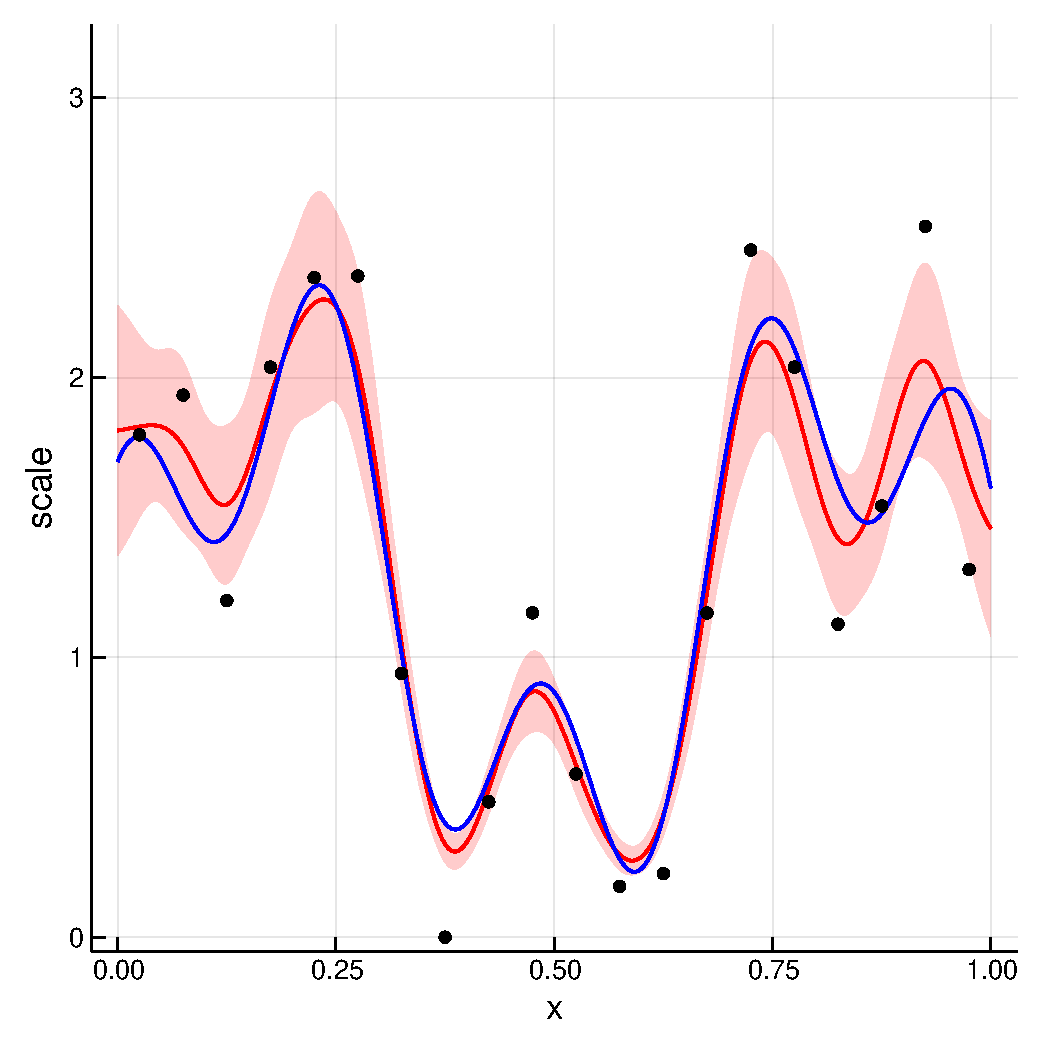
\includegraphics[width=\textwidth]{figures/scale/est-p1000-a20-se1.pdf}
      \caption{True and estimated scale function using 20 NRBFs}
    \end{subfigure}
  \end{tabular}
  \caption{Nonstationary scale parameter estimation for a 1D simulated random field. The isotropic Mat\'ern covariance with fixed $\ell=1$ and $\nu=1/2$ was used to generate 1,000 observations on a regular grid in $[0,1]$ with NRBF centers also on a regular grid. MLE computed using BFGS.}
  \label{}
\end{figure}

\begin{figure}[t!]
  \centering
  \begin{tabular}{ccc}
    \begin{subfigure}[t]{0.3\textwidth}
      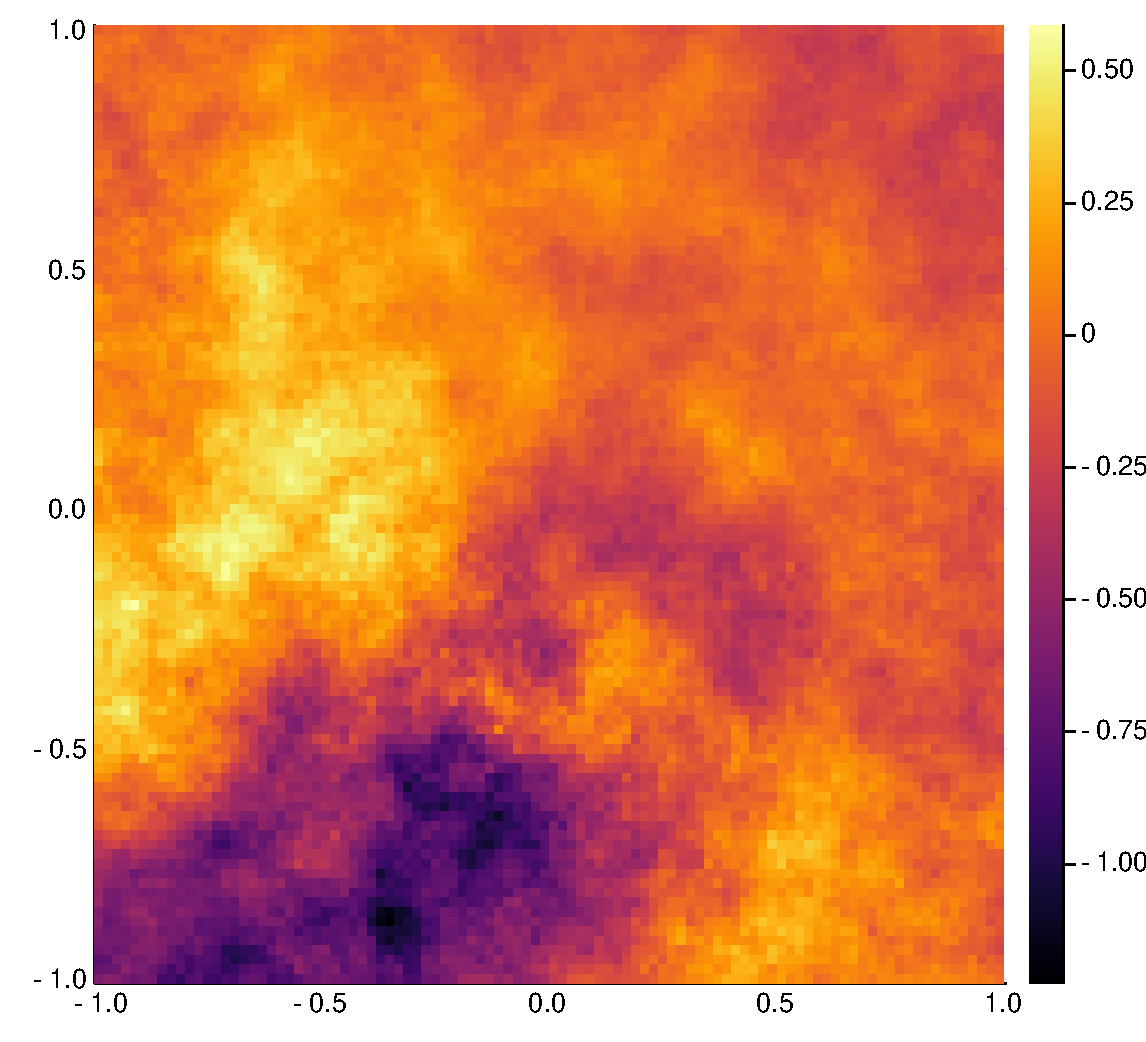
\includegraphics[width=\textwidth]{figures/isotropic/dat-nsr-p10000.pdf}
      \caption{Simulated random field}
    \end{subfigure} &
    \begin{subfigure}[t]{0.3\textwidth}
      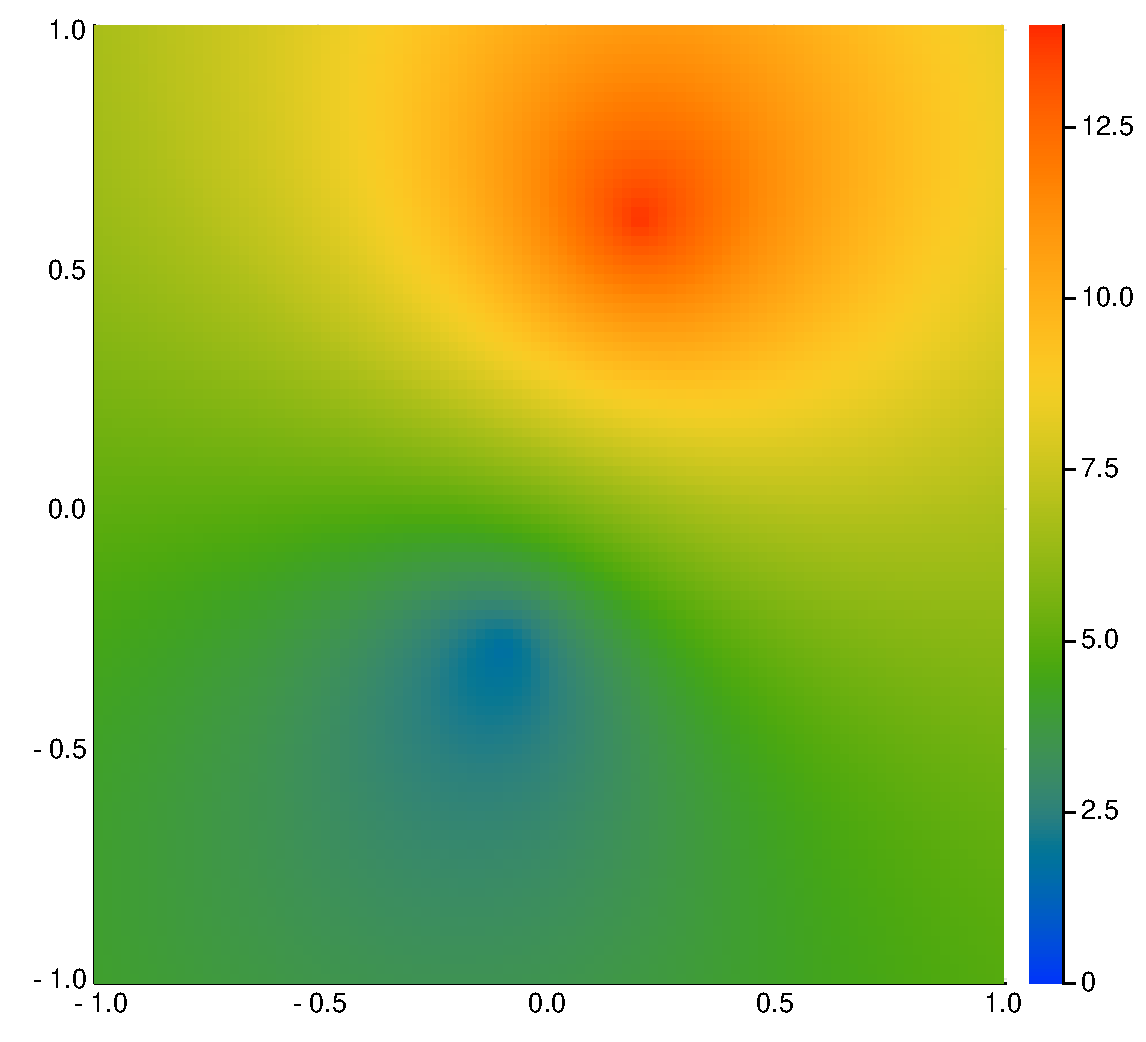
\includegraphics[width=\textwidth]{figures/isotropic/tru-nsr-p10000.pdf}
      \caption{True range function}
    \end{subfigure}
    & \\[4ex]
    &
    \multicolumn{2}{l}{
      \begin{subfigure}[t]{0.6\textwidth}
        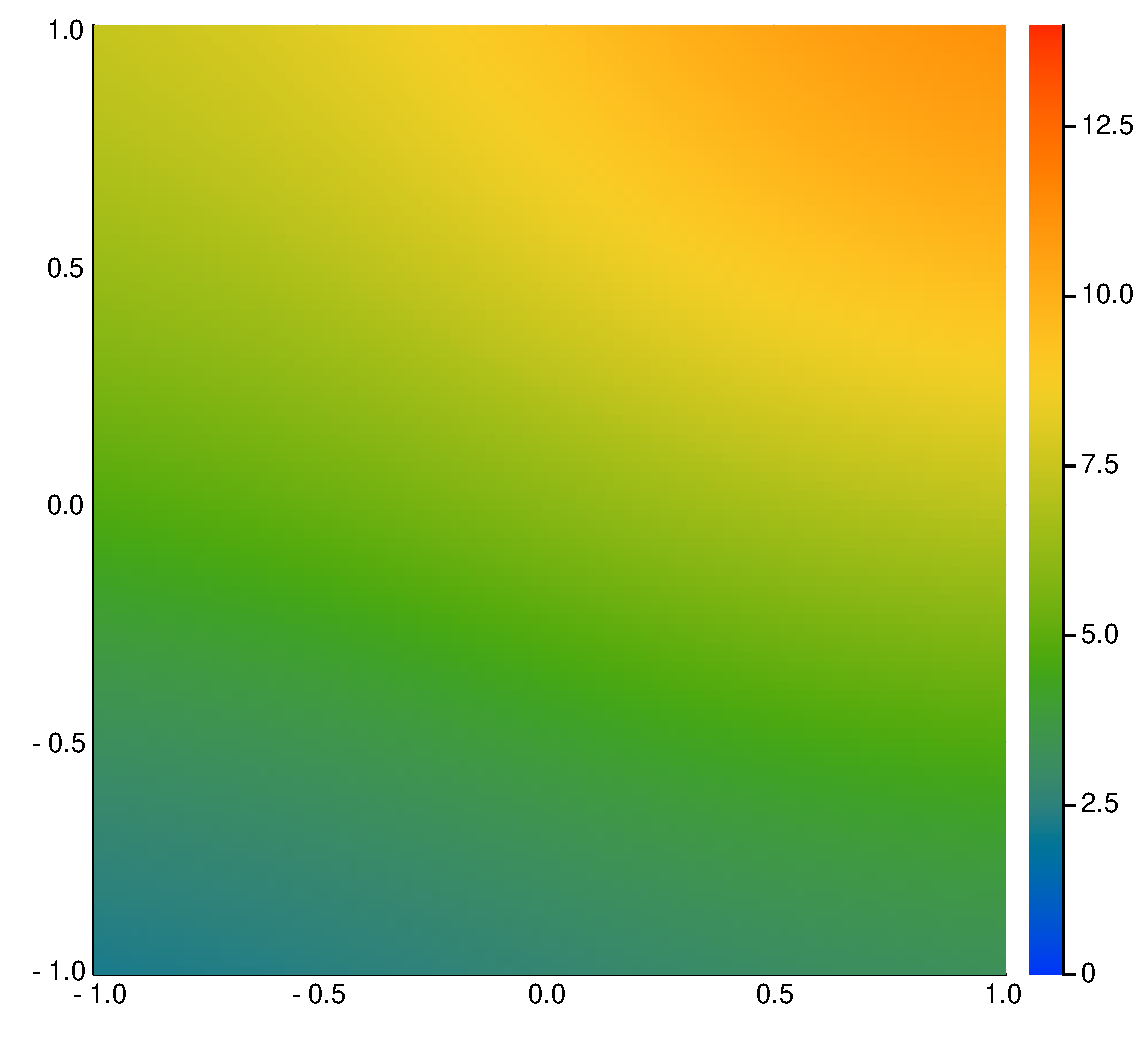
\includegraphics[width=0.5\textwidth]{figures/isotropic/est-nsr-p10000-a4.pdf}%
        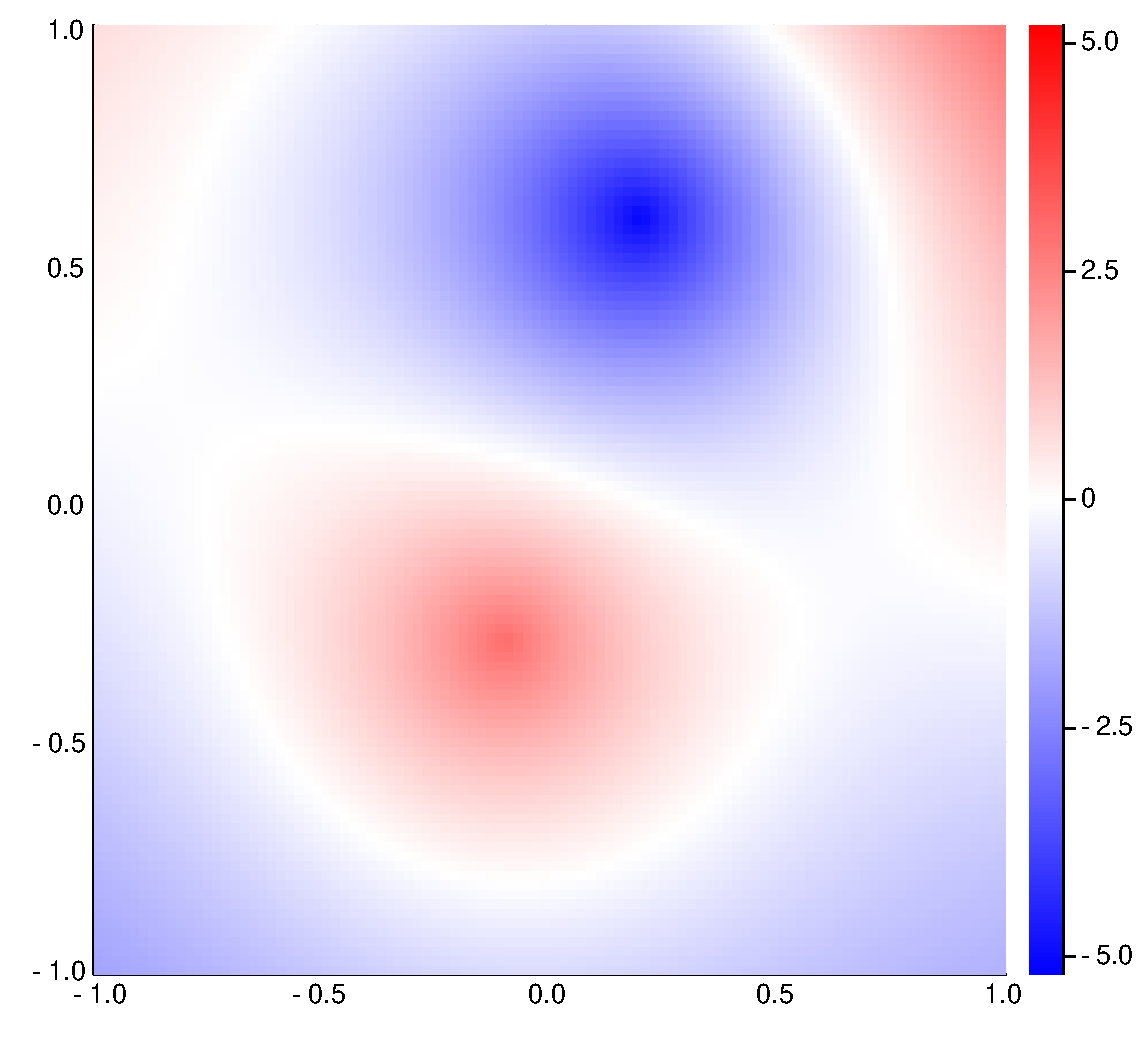
\includegraphics[width=0.5\textwidth]{figures/isotropic/err-nsr-p10000-a4.pdf}
        \caption{Estimated range function (left) and error (right) using 4 NRBFs}
      \end{subfigure}
    } \\[4ex]
    &
    \multicolumn{2}{l}{
      \begin{subfigure}[t]{0.6\textwidth}
        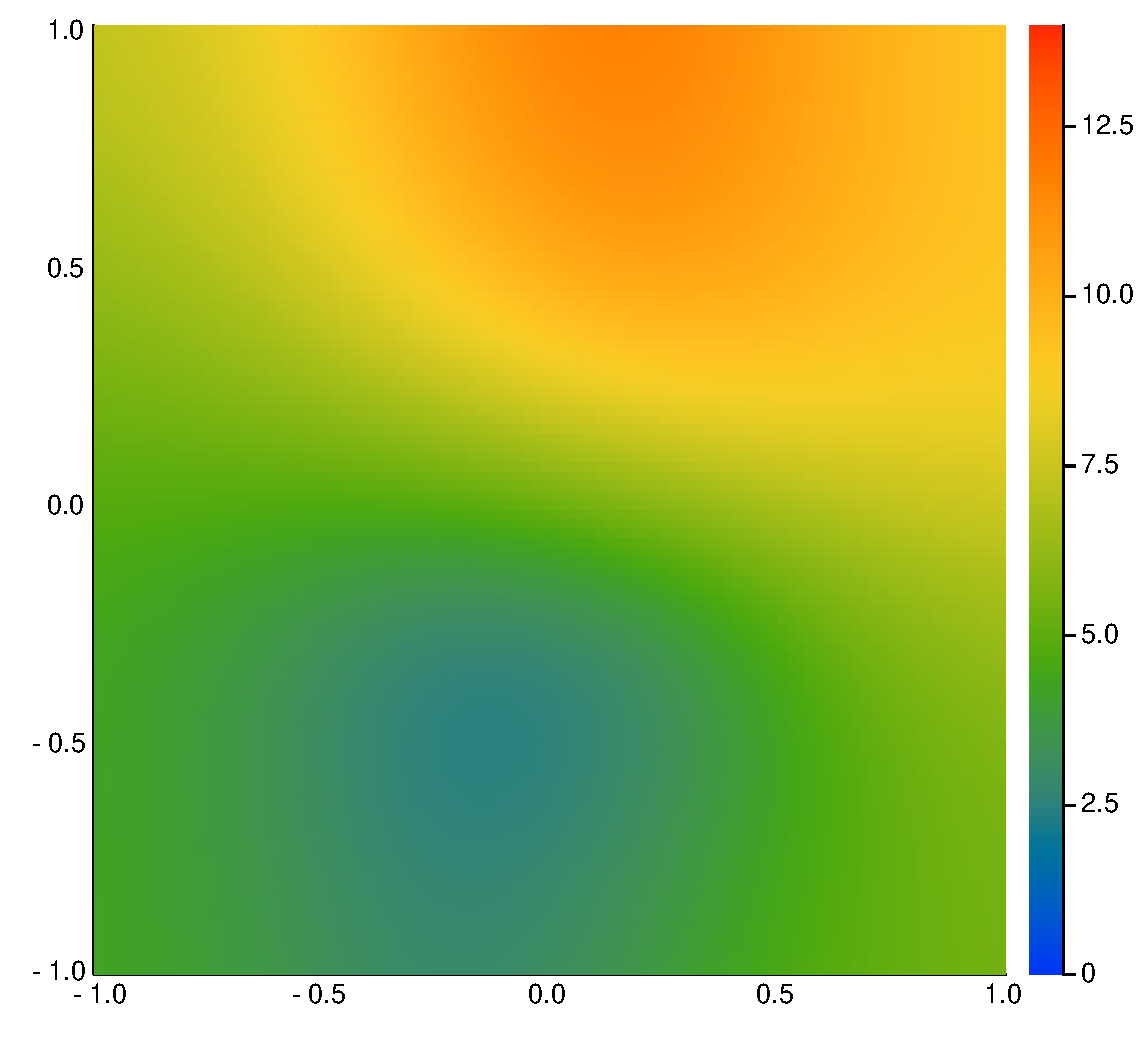
\includegraphics[width=0.5\textwidth]{figures/isotropic/est-nsr-p10000-a16.pdf}%
        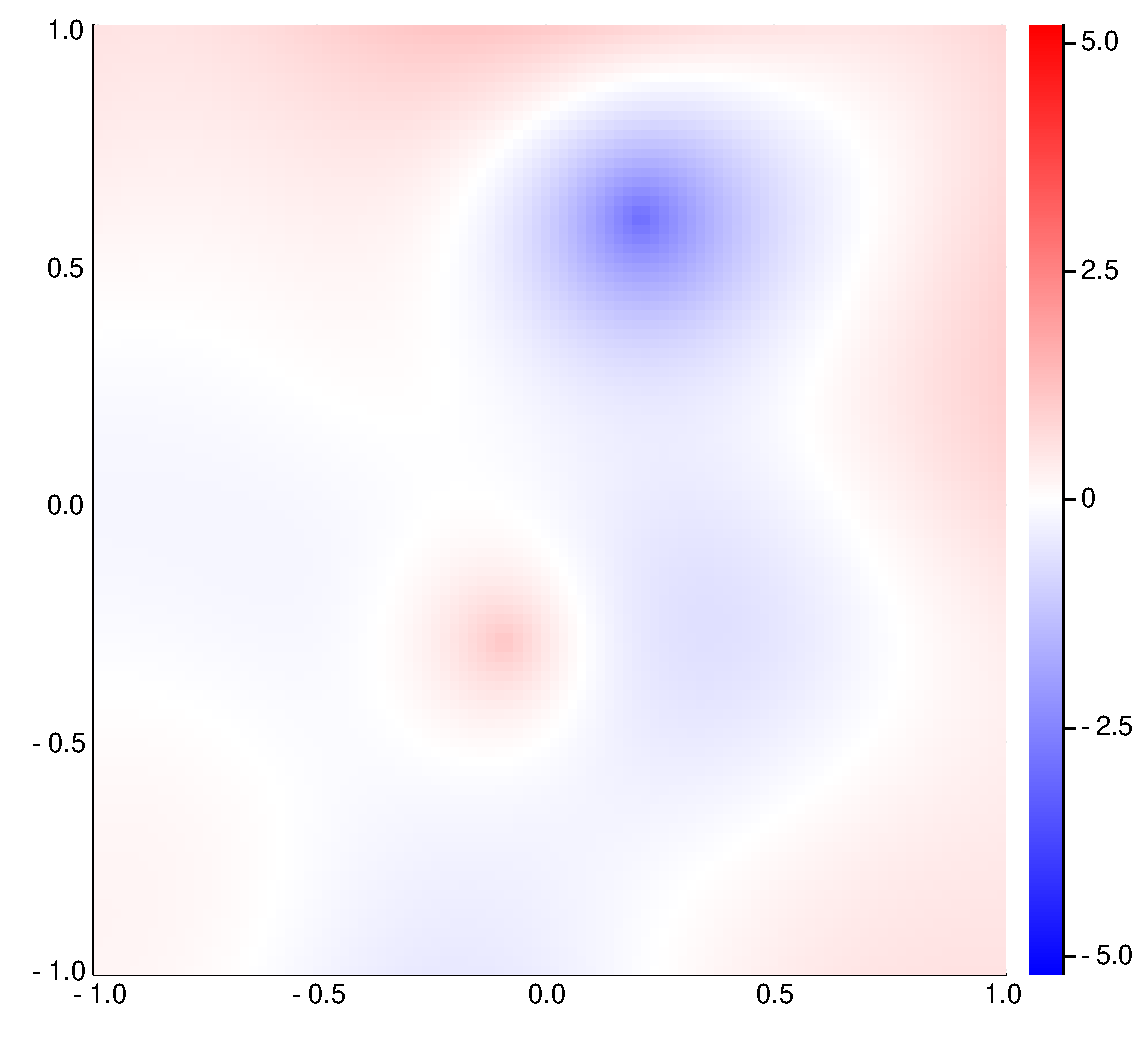
\includegraphics[width=0.5\textwidth]{figures/isotropic/err-nsr-p10000-a16.pdf}
        \caption{Estimated range function and error using 16 NRBFs}
      \end{subfigure}
    } \\[4ex]
    &
    \multicolumn{2}{l}{
      \begin{subfigure}[t]{0.6\textwidth}
        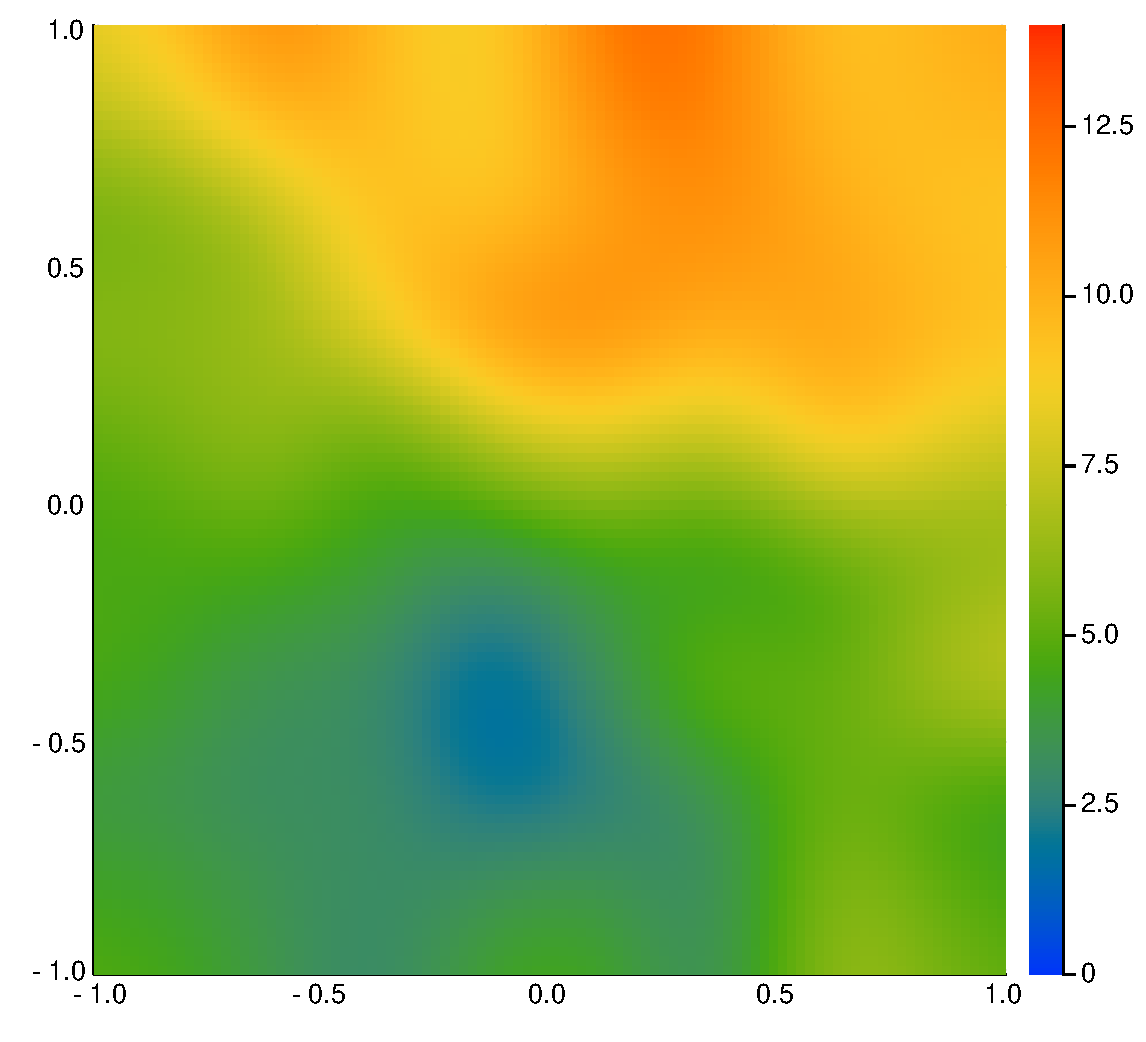
\includegraphics[width=0.5\textwidth]{figures/isotropic/est-nsr-p10000-a64.pdf}%
        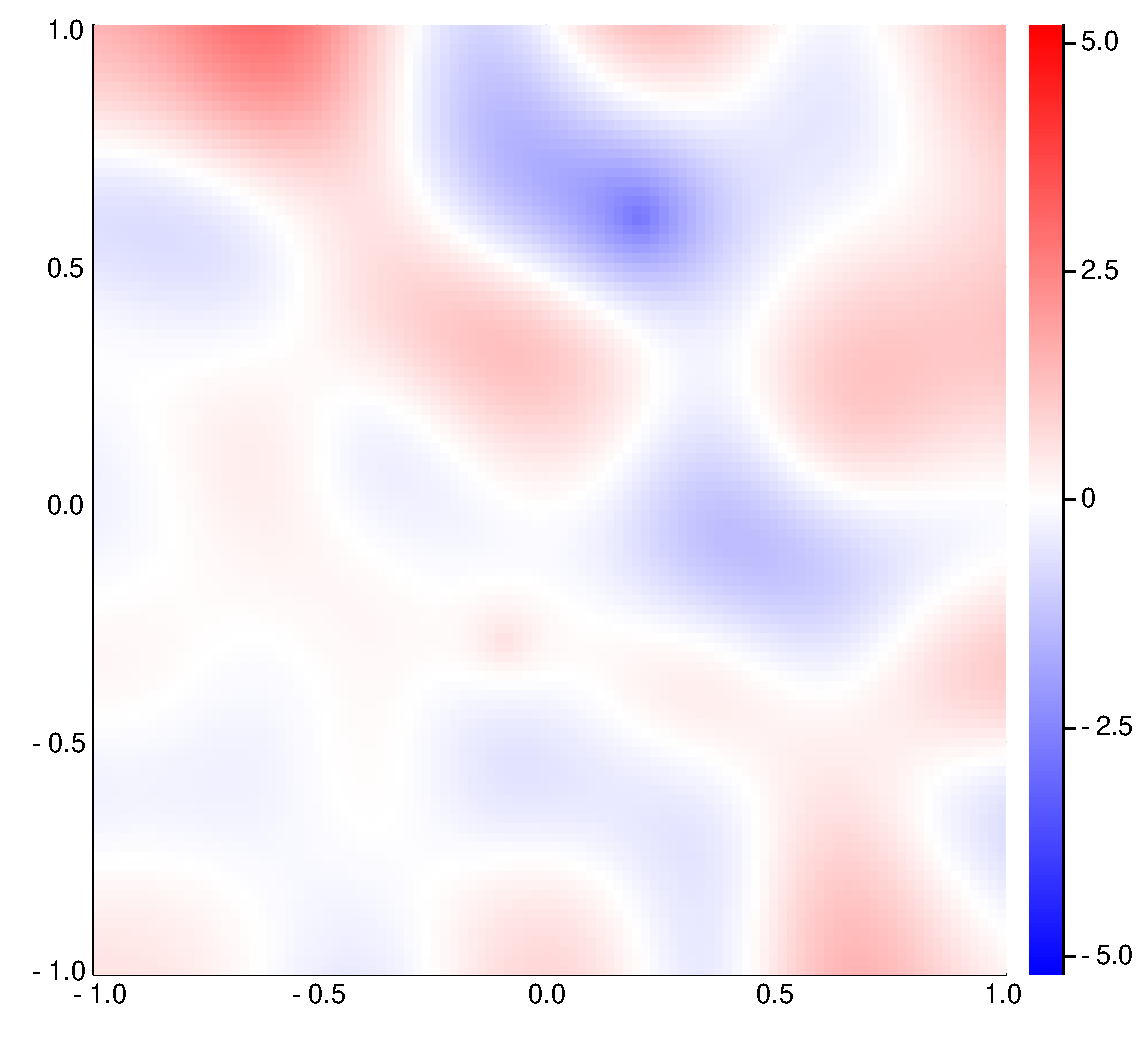
\includegraphics[width=0.5\textwidth]{figures/isotropic/err-nsr-p10000-a64.pdf}
        \caption{Estimated range function and error using 64 NRBFs}
      \end{subfigure}
    }
  \end{tabular}
  \caption{Nonstationary range parameter estimation for a 2D simulated random field. The isotropic Mat\'ern covariance with fixed $\sigma^2=1$ and $\nu=1/2$ was used to generate 10,000 observations on a regular grid in $[-1,1]^2$ with NRBF centers also on a regular grid. MLE computed using BFGS.}
  \label{}
\end{figure}

\bibliography{refs}{}
\bibliographystyle{plain}

\end{document}
